\documentclass{beamer}
\usepackage[utf8]{inputenc}
\usepackage[T1]{fontenc}
\usepackage{tikz}
\usepackage{utopia}
\usepackage[absolute,overlay]{textpos}
\usepackage{transparent}

\usetheme{Madrid}
\usecolortheme{default}

%------------------------------------------------------------
\title[Geode]
{Global analytics in the face of bandwidth and regulatory constraints}

\subtitle{Geode}

\author[Vulimiri et al., 2015]
{Ashish Vulimiri, Thomas Jungblut, Carlo Curino, Jitu Padhye, Brighten Godfrey, George Varghese}

\date[Big Data Infrastructure]
{Presented by Claudio Scheer}
%------------------------------------------------------------


%------------------------------------------------------------
\AtBeginSection[]
{
	\begin{frame}
		\frametitle{Table of Contents}
		\tableofcontents[currentsection]
	\end{frame}
}
%------------------------------------------------------------


\begin{document}

\frame{\titlepage}


\section{Overview}
%---------------------------------------------------------
\begin{frame}
	\frametitle{Wide-Area Big Data}

	\includegraphics[width=\textwidth]{./images/centralized.pdf}

	\begin{textblock}{1}(6.5,12)
		\includegraphics[height=1.8cm]{./images/internet-growth.png}
	\end{textblock}
\end{frame}

\begin{frame}
	\frametitle{Geode}

	\begin{itemize}
		\item SQL analytics over geo-distributed data;
		\item Support joins over geo-distributed data centers;
		\item ``What's the best join order?'' to reduce bandwidth;
		\item No attempt to minimize execution latency;
	\end{itemize}
\end{frame}
%---------------------------------------------------------


\section{Geode}
%---------------------------------------------------------
\begin{frame}
	\frametitle{Example}

	\begin{textblock}{11}(.5,12.5)
		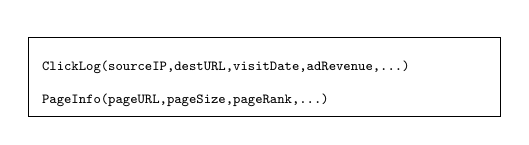
\begin{tikzpicture}
			\filldraw[fill=white,draw=black] (0,0) rectangle (6,1) node[above left,pos=0,yshift=0cm,xshift=3.3cm,text width=3cm] {
					{
							\tiny
							\texttt{ClickLog(sourceIP,destURL,visitDate,adRevenue,...)}
							\texttt{PageInfo(pageURL,pageSize,pageRank,...)}
						}
				};
		\end{tikzpicture}
	\end{textblock}

	\includegraphics[width=\textwidth]{./images/geode.pdf}
\end{frame}

\begin{frame}
	\frametitle{Example - centralized}

	{\transparent{0.1}\includegraphics[width=\textwidth]{./images/centralized.png}}

	\begin{textblock}{11}(1.5,3.5)
		SELECT sourceIP, sum(adRevenue), avg(pageRank)
		\break
		FROM ClickLog cl
		\break
		JOIN PageInfo pi ON cl.destURL = pi.pageURL
		\break
		WHERE pi.pageCategory = `Entertainment'
		\break
		GROUP BY sourceIP
		\break
		HAVING sum(adRevenue) >= 100;
	\end{textblock}

	\begin{textblock}{7}(1.5,11)
		1B users
		\break
		6 pages visited per user/day
		\break
		200 bytes per ClickLog row
		\hline
		\vspace{4px}
		= 1.2 TB
	\end{textblock}
\end{frame}

\begin{frame}
	\frametitle{Example - Geode}

	{\transparent{0.1}\includegraphics[width=\textwidth]{./images/geode.png}}

	\begin{textblock}{11}(1.5,3.5)
		SELECT sourceIP, sum(adRevenue), avg(pageRank)
		\break
		FROM ClickLog cl
		\break
		JOIN PageInfo pi ON cl.destURL = pi.pageURL
		\break
		WHERE pi.pageCategory = `Entertainment'
		\break
		GROUP BY sourceIP
		\break
		HAVING sum(adRevenue) >= 100;
	\end{textblock}

	\begin{textblock}{7}(1.5,10)
		1B users
		\break
		100M pages visited per day
		\break
		each q1 tuple is 20 bytes
		\break
		each q2, q3, q4 tuple is 12 bytes
		\hline
		\vspace{4px}
		= 14 GB
	\end{textblock}
\end{frame}

\begin{frame}
	\frametitle{Example - Geode}

	\includegraphics[width=\textwidth]{./images/geode-execution-plan.png}
\end{frame}

\begin{frame}
	\frametitle{Architecture}

	\includegraphics[width=\textwidth]{./images/architecture.png}
\end{frame}

\begin{frame}
	\frametitle{Query cache}

	\includegraphics[width=\textwidth]{./images/geode-cache.png}
\end{frame}

\begin{frame}
	\frametitle{Results}

	\begin{itemize}
		\item Centralized approach performs better when update rates are low;
		\item At high update rates, caching is ineffective;
		\item Distributed execution outperformed the centralized approach in four of six workloads (250x - 360x);
	\end{itemize}
\end{frame}

\begin{frame}
	\frametitle{Open challenges}

	\begin{itemize}
		\item Latency;
		\item They limit where data can be copied, but not data movement through queries;
		\item Support for other data models, such as MapReduce;
	\end{itemize}
\end{frame}
%---------------------------------------------------------

\end{document}
